\documentclass[english,hidelinks, 11 pt, class=report,crop=false]{standalone}
\usepackage[T1]{fontenc}
%\usepackage[utf8]{inputenc}
\usepackage{lmodern} % load a font with all the characters
\usepackage{geometry}
\geometry{verbose,paperwidth=16.1 cm, paperheight=24 cm, inner=2.3cm, outer=1.8 cm, bmargin=2cm, tmargin=1.8cm}
\setlength{\parindent}{0bp}
\usepackage{import}
\usepackage[subpreambles=false]{standalone}
\usepackage{amsmath}
\usepackage{amssymb}
\usepackage{esint}
\usepackage{babel}
\usepackage{tabu}
\makeatother
\makeatletter

\usepackage{titlesec}
\usepackage{ragged2e}
\RaggedRight
\raggedbottom
\frenchspacing

\usepackage{graphicx}
\usepackage{float}
\usepackage{subfig}
\usepackage{placeins}
\usepackage{cancel}
\usepackage{framed}
\usepackage{wrapfig}
\usepackage[subfigure]{tocloft}
\usepackage[font=footnotesize,labelfont=sl]{caption} % Figure caption
\usepackage{bm}
\usepackage[dvipsnames, table]{xcolor}
\definecolor{shadecolor}{rgb}{0.105469, 0.613281, 1}
\colorlet{shadecolor}{Emerald!15} 
\usepackage{icomma}
\makeatother
\usepackage[many]{tcolorbox}
\usepackage{multicol}
\usepackage{stackengine}

\usepackage{esvect} %For vectors with capital letters

% For tabular
\usepackage{array}
\usepackage{multirow}
\usepackage{longtable} %breakable table

% Ligningsreferanser
\usepackage{mathtools} % for mathclap
%\mathtoolsset{showonlyrefs}

% sections without numbering in toc
\newcommand\tsec[1]{\phantomsection \addcontentsline{toc}{section}{#1}
	\section*{#1}}

% index
\usepackage{imakeidx}
\makeindex[title=Indeks]

%Footnote:
\usepackage[bottom, hang, flushmargin]{footmisc}
\usepackage{perpage} 
\MakePerPage{footnote}
\addtolength{\footnotesep}{2mm}
\renewcommand{\thefootnote}{\arabic{footnote}}
\renewcommand\footnoterule{\rule{\linewidth}{0.4pt}}
\renewcommand{\thempfootnote}{\arabic{mpfootnote}}

%colors
\definecolor{c1}{cmyk}{0,0.5,1,0}
\definecolor{c2}{cmyk}{1,0.25,1,0}
\definecolor{n3}{cmyk}{1,0.,1,0}
\definecolor{neg}{cmyk}{1,0.,0.,0}


\newcommand{\nreq}[1]{
\begin{equation}
	#1
\end{equation}
}


% Equation comments
\newcommand{\cm}[1]{\llap{\color{blue} #1}}


\usepackage[inline]{enumitem}
\newcounter{rg}
\numberwithin{rg}{chapter}


\newcommand{\reg}[2][]{\begin{tcolorbox}[boxrule=0.3 mm,arc=0mm,colback=blue!3] {\refstepcounter{rg}\phantomsection \large \textbf{\therg \;#1} \vspace{5 pt}}\newline #2  \end{tcolorbox}\vspace{-5pt}}
\newcommand{\regdef}[2][]{\begin{tcolorbox}[boxrule=0.3 mm,arc=0mm,colback=blue!3] {\refstepcounter{rg}\phantomsection \large \textbf{\therg \;#1} \vspace{5 pt}}\newline #2  \end{tcolorbox}\vspace{-5pt}}
\newcommand{\words}[1]{\begin{tcolorbox}[boxrule=0.3 mm,arc=0mm,colback=teal!3] #1  \end{tcolorbox}\vspace{-5pt}}

\newcommand\alg[1]{\begin{align*} #1 \end{align*}}

\newcommand\eks[2][]{\begin{tcolorbox}[boxrule=0.3 mm,arc=0mm,enhanced jigsaw,breakable,colback=green!3] {\large \textbf{\ekstitle #1} \vspace{5 pt}\\} #2 \end{tcolorbox}\vspace{-5pt} }

\newcommand{\st}[1]{\begin{tcolorbox}[boxrule=0.0 mm,arc=0mm,enhanced jigsaw,breakable,colback=yellow!12]{ #1} \end{tcolorbox}}

\newcommand{\spr}[1]{\begin{tcolorbox}[boxrule=0.3 mm,arc=0mm,enhanced jigsaw,breakable,colback=yellow!7] {\large \textbf{\sprtitle} \vspace{5 pt}\\} #1 \end{tcolorbox}\vspace{-5pt} }

\newcommand{\sym}[1]{\colorbox{blue!15}{#1}}

\newcommand{\info}[2]{\begin{tcolorbox}[boxrule=0.3 mm,arc=0mm,enhanced jigsaw,breakable,colback=cyan!6] {\large \textbf{#1} \vspace{5 pt}\\} #2 \end{tcolorbox}\vspace{-5pt} }

\newcommand\algv[1]{\vspace{-11 pt}\begin{align*} #1 \end{align*}}

\newcommand{\regv}{\vspace{5pt}}
\newcommand{\mer}{\textsl{\note}: }
\newcommand{\mers}[1]{{\footnotesize \mer #1}}
\newcommand\vsk{\vspace{11pt}}
\newcommand{\tbs}{\vspace{5pt}}
\newcommand\vs{\vspace{-11pt}}
\newcommand\vsb{\vspace{-16pt}}
\newcommand\br{\\[5 pt]}
\newcommand{\figp}[1]{../fig/#1}
\newcommand\algvv[1]{\vs\vs\begin{align*} #1 \end{align*}}
\newcommand{\y}[1]{$ {#1} $}
\newcommand{\os}{\\[5 pt]}
\newcommand{\prbxl}[2]{
\parbox[l][][l]{#1\linewidth}{#2
	}}
\newcommand{\prbxr}[2]{\parbox[r][][l]{#1\linewidth}{
		\setlength{\abovedisplayskip}{5pt}
		\setlength{\belowdisplayskip}{5pt}	
		\setlength{\abovedisplayshortskip}{0pt}
		\setlength{\belowdisplayshortskip}{0pt} 
		\begin{shaded}
			\footnotesize	#2 \end{shaded}}}
\newcommand{\fgbxr}[2]{
	\parbox[r][][l]{#1\linewidth}{#2
}}		

\renewcommand{\cfttoctitlefont}{\Large\bfseries}
\setlength{\cftaftertoctitleskip}{0 pt}
\setlength{\cftbeforetoctitleskip}{0 pt}

\newcommand{\bs}{\\[3pt]}
\newcommand{\vn}{\\[6pt]}
\newcommand{\fig}[1]{\begin{figure}[H]
		\centering
		\includegraphics[]{\figp{#1}}
\end{figure}}

\newcommand{\figc}[2]{\begin{figure}
		\centering
		\includegraphics[]{\figp{#1}}
		\caption{#2}
\end{figure}}
\newcommand{\arc}[1]{{
		\setbox9=\hbox{#1}%
		\ooalign{\resizebox{\wd9}{\height}{\texttoptiebar{\phantom{A}}}\cr\textit{#1}}}}

\newcommand{\sectionbreak}{\clearpage} % New page on each section

\newcommand{\nn}[1]{
\begin{equation*}
	#1
\end{equation*}
}

\newcommand{\enh}[1]{\,\textrm{#1}}

%asin, atan, acos
\DeclareMathOperator{\atan}{atan}
\DeclareMathOperator{\acos}{acos}
\DeclareMathOperator{\asin}{asin}

% Comments % old cm, ggb cm is new
%\newcommand{\cm}[1]{\llap{\color{blue} #1}}

%%%

\newcommand\fork[2]{\begin{tcolorbox}[boxrule=0.3 mm,arc=0mm,enhanced jigsaw,breakable,colback=yellow!7] {\large \textbf{#1 (\expl)} \vspace{5 pt}\\} #2 \end{tcolorbox}\vspace{-5pt} }
 
%colors
\newcommand{\colr}[1]{{\color{red} #1}}
\newcommand{\colb}[1]{{\color{blue} #1}}
\newcommand{\colo}[1]{{\color{orange} #1}}
\newcommand{\colc}[1]{{\color{cyan} #1}}
\definecolor{projectgreen}{cmyk}{100,0,100,0}
\newcommand{\colg}[1]{{\color{projectgreen} #1}}

% Methods
\newcommand{\metode}[2]{
	\textsl{#1} \\[-8pt]
	\rule{#2}{0.75pt}
}

%Opg
\newcommand{\abc}[1]{
	\begin{enumerate}[label=\alph*),leftmargin=18pt]
		#1
	\end{enumerate}
}
\newcommand{\abcs}[2]{
	\begin{enumerate}[label=\alph*),start=#1,leftmargin=18pt]
		#2
	\end{enumerate}
}
\newcommand{\abcn}[1]{
	\begin{enumerate}[label=\arabic*),leftmargin=18pt]
		#1
	\end{enumerate}
}
\newcommand{\abch}[1]{
	\hspace{-2pt}	\begin{enumerate*}[label=\alph*), itemjoin=\hspace{1cm}]
		#1
	\end{enumerate*}
}
\newcommand{\abchs}[2]{
	\hspace{-2pt}	\begin{enumerate*}[label=\alph*), itemjoin=\hspace{1cm}, start=#1]
		#2
	\end{enumerate*}
}

% Exercises


\newcounter{opg}
\numberwithin{opg}{section}

\newcounter{grub}
\numberwithin{opg}{section}
\newcommand{\op}[1]{\vspace{15pt} \refstepcounter{opg}\large \textbf{\color{blue}\theopg} \vspace{2 pt} \label{#1} \\}
\newcommand{\eksop}[2]{\vspace{15pt} \refstepcounter{opg}\large \textbf{\color{blue}\theopg} (#1) \vspace{2 pt} \label{#2} \\}

\newcommand{\nes}{\stepcounter{section}
	\setcounter{opg}{0}}
\newcommand{\opr}[1]{\vspace{3pt}\textbf{\ref{#1}}}
\newcommand{\oeks}[1]{\begin{tcolorbox}[boxrule=0.3 mm,arc=0mm,colback=white]
		\textit{\ekstitle: } #1	  
\end{tcolorbox}}
\newcommand\opgeks[2][]{\begin{tcolorbox}[boxrule=0.1 mm,arc=0mm,enhanced jigsaw,breakable,colback=white] {\footnotesize \textbf{\ekstitle #1} \\} \footnotesize #2 \end{tcolorbox}\vspace{-5pt} }


% tag exercises
\newcommand{\tagop}[1]{ 
{\small \color{Gray} #1} \os
}

% License
\newcommand{\lic}{
This book is part of the \net{https://sindrsh.github.io/openmathbooks/}{OpenMathBooks} project. OpenMathBooks © 2022 by Sindre Sogge Heggen is licensed under CC BY-NC-SA 4.0. To view a copy of this license, visit \net{http://creativecommons.org/licenses/by-nc-sa/4.0/}{http://creativecommons.org/licenses/by-nc-sa/4.0/}}

%referances
\newcommand{\net}[2]{{\color{blue}\href{#1}{#2}}}
\newcommand{\hrs}[2]{\hyperref[#1]{\color{blue}#2 \ref*{#1}}}
\newcommand{\refunnbr}[2]{\hyperref[#1]{\color{blue}#2}}


\newcommand{\openmath}{\net{https://sindrsh.github.io/openmathbooks/}{OpenMathBooks}}
\newcommand{\am}{\net{https://sindrsh.github.io/FirstPrinciplesOfMath/}{AM1}}
\newcommand{\mb}{\net{https://sindrsh.github.io/FirstPrinciplesOfMath/}{MB}}
\newcommand{\tmen}{\net{https://sindrsh.github.io/FirstPrinciplesOfMath/}{TM1}}
\newcommand{\tmto}{\net{https://sindrsh.github.io/FirstPrinciplesOfMath/}{TM2}}
\newcommand{\amto}{\net{https://sindrsh.github.io/FirstPrinciplesOfMath/}{AM2}}
\newcommand{\eksbm}{
\footnotesize
Dette er opppgaver som har blitt gitt ved sentralt utformet eksamen i Norge. Oppgavene er laget av Utdanningsdirektoratet. Forkortelser i parantes viser til følgende:
\begin{center}
	\begin{tabular}{c|c}
		E & Eksempeloppgave \\
		V/H & Eksamen fra vårsemesteret/høstsemesteret\\
		G/1P/1T/R1/R2 & Fag  \\
		XX & År 20XX \\
		D1/D2 & Del 1/Del 2
	\end{tabular}
\end{center}
Tekst og innhold kan her være noe endret i forhold til originalen.
}

%Excel og GGB:

\newcommand{\g}[1]{\begin{center} {\tt #1} \end{center}}
\newcommand{\gv}[1]{\begin{center} \vspace{-11 pt} {\tt #1}  \end{center}}
\newcommand{\cmds}[2]{{\tt #1}\\
	#2}

% outline word
\newcommand{\outl}[1]{{\boldmath \color{teal}\textbf{#1}}}
%line to seperate examples
\newcommand{\linje}{\rule{\linewidth}{1pt} }


%Vedlegg
\newcounter{vedl}
\newcounter{vedleq}
\renewcommand\thevedl{\Alph{vedl}}	
\newcommand{\nreqvd}{\refstepcounter{vedleq}\tag{\thevedl \thevedleq}}

%%% Writing code

\usepackage{listings}


\definecolor{codegreen}{rgb}{0,0.6,0}
\definecolor{codegray}{rgb}{0.5,0.5,0.5}
\definecolor{codepurple}{rgb}{0.58,0,0.82}
\definecolor{backcolour}{rgb}{0.95,0.95,0.92}

\newcommand{\pymet}[1]{{\ttfamily\color{magenta} #1}}
\newcommand{\pytype}[1]{{\ttfamily\color{codepurple} #1}}

\lstdefinestyle{mystyle}{
	backgroundcolor=\color{backcolour},   
	commentstyle=\color{codegreen},
	keywordstyle=\color{magenta},
	numberstyle=\tiny\color{codegray},
	stringstyle=\color{codepurple},
	basicstyle=\ttfamily\footnotesize,
	breakatwhitespace=false,         
	breaklines=true,                 
	captionpos=b,                    
	keepspaces=true,                 
	numbers=left,                    
	numbersep=5pt,                  
	showspaces=false,                
	showstringspaces=false,
	showtabs=false,                  
	tabsize=2,
	inputencoding=utf8,
	extendedchars=true,
	literate= {
		{å}{{\aa}}1 
		{æ}{{\ae}}1 
		{ø}{{\o}}1
	}
}

\lstset{style=mystyle}

\newcommand{\python}[1]{
\begin{tcolorbox}[boxrule=0.3 mm,arc=0mm,colback=white]
\lstinputlisting[language=Python]{#1}
\end{tcolorbox}}
\newcommand{\pythonut}[2]{
\begin{tcolorbox}[boxrule=0.3 mm,arc=0mm,colback=white]
\small 
%\textbf{Kode}
\lstinputlisting[language=Python]{#1}	
\vspace{11pt}
\textbf{Utdata} \\ \ttfamily
#2
\end{tcolorbox}}
%%%

%page number
%\usepackage{fancyhdr}
%\pagestyle{fancy}
%\fancyhf{}
%\renewcommand{\headrule}{}
%\fancyhead[RO, LE]{\thepage}

\usepackage{datetime2}
%%\usepackage{sansmathfonts} for dyslexia-friendly math
\usepackage[]{hyperref}


% note
\newcommand{\note}{Note}
\newcommand{\notesm}[1]{{\footnotesize \textsl{\note:} #1}}
\newcommand{\selos}{See the solutions manual.}

\newcommand{\texandasy}{The text is written in \LaTeX\ and the figures are made with the aid of Asymptote.}

\newcommand{\rknut}{Calculate.}
\newcommand\sv{\vsk \textbf{Answer} \vspace{4 pt}\\}
\newcommand{\ekstitle}{Example }
\newcommand{\sprtitle}{The language box}
\newcommand{\expl}{explanation}

% answers
\newcommand{\mulansw}{\notesm{Multiple possible answers.}}	
\newcommand{\faskap}{Chapter}

% exercises
\newcommand{\opgt}{\newpage \phantomsection \addcontentsline{toc}{section}{Exercises} \section*{Exercises for Chapter \thechapter}\vs \setcounter{section}{1}}

\newcommand{\grubop}[1]{\vspace{15pt} \refstepcounter{grub}\large \textbf{\color{blue} Ponder \thegrub} \vspace{2 pt} \label{#1} \\}
\newcommand{\grubr}[1]{\vspace{3pt}\textbf{Ponder \ref{#1}}}


% references
\newcommand{\reftab}[1]{\hrs{#1}{Table}}
\newcommand{\rref}[1]{\hrs{#1}{Rule}}
\newcommand{\dref}[1]{\hrs{#1}{Definition}}
\newcommand{\refkap}[1]{\hrs{#1}{Chapter}}
\newcommand{\refsec}[1]{\hrs{#1}{Section}}
\newcommand{\refdsec}[1]{\hrs{#1}{Subsection}}
\newcommand{\refved}[1]{\hrs{#1}{Appendix}}
\newcommand{\eksref}[1]{\textsl{#1}}
\newcommand\fref[2][]{\hyperref[#2]{\textsl{Figure \ref*{#2}#1}}}
\newcommand{\refop}[1]{{\color{blue}Exercise \ref{#1}}}
\newcommand{\refops}[1]{{\color{blue}Exercise \ref{#1}}}

%%% SECTION HEADLINES %%%

% Our numbers
\newcommand{\likteikn}{The equal sign}
\newcommand{\talsifverd}{Numbers, digits and values}
\newcommand{\koordsys}{Coordinate systems}

% Calculations
\newcommand{\adi}{Addition}
\newcommand{\sub}{Subtraction}
\newcommand{\gong}{Multiplication}
\newcommand{\del}{Division}

%Factorization and order of operations
\newcommand{\fak}{Factorization}
\newcommand{\rrek}{Order of operations}

%Fractions
\newcommand{\brgrpr}{Introduction}
\newcommand{\brvu}{Values, expanding and simplifying}
\newcommand{\bradsub}{Addition and subtraction}
\newcommand{\brgngheil}{Fractions multiplied by integers}
\newcommand{\brdelheil}{Fractions divided by integers}
\newcommand{\brgngbr}{Fractions multiplied by fractions}
\newcommand{\brkans}{Cancelation of fractions}
\newcommand{\brdelmbr}{Division by fractions}
\newcommand{\Rasjtal}{Rational numbers}

%Negative numbers
\newcommand{\negintro}{Introduction}
\newcommand{\negrekn}{The elementary operations}
\newcommand{\negmeng}{Negative numbers as amounts}

%Calculation methods
\newcommand{\delmedtihundre}{Deling med 10, 100, 1\,000 osv.}

% Geometry 1
\newcommand{\omgr}{Terms}
\newcommand{\eignsk}{Attributes of triangles and quadrilaterals}
\newcommand{\omkr}{Perimeter}
\newcommand{\area}{Area}

%Algebra 
\newcommand{\algintro}{Introduction}
\newcommand{\pot}{Powers}
\newcommand{\irrasj}{Irrational numbers}

%Equations
\newcommand{\ligintro}{Introduction}
\newcommand{\liglos}{Solving with the elementary operations}
\newcommand{\ligloso}{Solving with elementary operations summarized}

%Functions
\newcommand{\fintro}{Introduction}
\newcommand{\lingraf}{Linear functions and graphs}

%Geometry 2
\newcommand{\geoform}{Formulas of area and perimeter}
\newcommand{\kongogsim}{Congruent and similar triangles}
\newcommand{\geofork}{Explanations}

% Names of rules
\newcommand{\adkom}{Addition is commutative}
\newcommand{\gangkom}{Multiplication is commutative}
\newcommand{\brdef}{Fractions as rewriting of division}
\newcommand{\brtbr}{Fractions multiplied by fractions}
\newcommand{\delmbr}{Fractions divided by fractions}
\newcommand{\gangpar}{Distributive law}
\newcommand{\gangparsam}{Paranthesis multiplied together}
\newcommand{\gangmnegto}{Multiplication by negative numbers I}
\newcommand{\gangmnegtre}{Multiplication by negative numbers II}
\newcommand{\konsttre}{Unique construction of triangles}
\newcommand{\kongtre}{Congruent triangles}
\newcommand{\topv}{Vertical angles}
\newcommand{\trisum}{The sum of angles in a triangle}
\newcommand{\firsum}{The sum of angles in a quadrilateral}
\newcommand{\potgang}{Multiplication by powers}
\newcommand{\potdivpot}{Division by powers}
\newcommand{\potanull}{The special case of \boldmath $a^0$}
\newcommand{\potneg}{Powers with negative exponents}
\newcommand{\potbr}{Fractions as base}
\newcommand{\faktgr}{Factors as base}
\newcommand{\potsomgrunn}{Powers as base}
\newcommand{\arsirk}{The area of a circle}
\newcommand{\artrap}{The area of a trapezoid}
\newcommand{\arpar}{The area of a parallelogram}
\newcommand{\pyt}{Pythagoras's theorem}
\newcommand{\forform}{Ratios in similar triangles}
\newcommand{\vilkform}{Terms of similar triangles}
\newcommand{\omkrsirk}{The perimeter of a circle (and the value of $ \bm \pi $)}
\newcommand{\artri}{The area of a triangle}
\newcommand{\arrekt}{The area of a rectangle}
\newcommand{\liknflyt}{Moving terms across the equal sign}
\newcommand{\funklin}{Linear functions}



\begin{document}
\section{Fundamental Principle}
The fundamental principle behind probability theory is that we inquire about the number of \outl{favorable outcomes} in a set of \outl{possible outcomes}. The probability of an \outl{event} is then determined as a ratio between these two.\os
	
\reg[Probability of an Event \label{grnprsp}]{\vs
\[ \text{probability of an event}= \frac{\text{number of favorable outcomes}}{\text{number of possible outcomes}} \]	
}\vsk

When we roll a dice, we call 'getting a four' an event. Since a dice has six different sides, there are six possible outcomes.
\fig{san1}
If we want to 'get a four,' there is only 1 out of these 6 outcomes that gives us what we want, so
\[\text{probability of 'getting a four'}=\frac{1}{6} \]
\prbxl{0.6}{To avoid long expressions, we often use single letters to represent an event. Instead of writing 'getting a four,' we can use the letter \textit{F}, and to indicate that we are talking about the probability of an event, we use the letter \textit{P}.}\qquad \prbxr{0.3}{$ P $ comes from the word \textit{probability}.} \vsk

When we write $P(S)$, this means 'the probability of getting a four':
\[ P(S)=\frac{1}{6} \]
What about the opposite, i.e., the probability of \textsl{not} getting a four? To express that something is the opposite of an event, we put a line over the name. So, we write the event 'not getting a four' as $ \bar{F} $. 'Not getting a four' is the same as 'getting \textsl{either} a one, a two, a three, a five, \textsl{or} a six,' which means this event has 5 favorable outcomes. That means
\[ P(\bar{S})=\frac{5}{6} \]
\reg[Symbols for Probability]{
	$ P(A) $ is the probability that event $ A $ occurs. \vsk
	$ A $ and $ \bar{A} $ are opposite events. \vsk
	$ P(\bar{A}) $ is the probability that $ A $ \textsl{does not} occur, and vice versa.
}
\info{Note!}{
	In general, it's a good practice to simplify fractions when possible. However, in probability theory, it often pays off to leave fractions in their current form. Therefore, you will notice that many fractions in the upcoming sections could have been simplified.
}
\section{Events with and without common outcomes}
\subsection{Events without common outcomes} \vspace{-5pt}
\prbxl{0.6}{Let's call the event 'rolling a three' (on a dice) as \textit{T}. The event 'rolling a three \textsl{or} a four' is then written as $ T\cup F $.} \qquad
\prbxr{0.3}{The symbol \sym{$ \cup $} is called \textit{union}.}
There are 2 out of 6 sides on a dice that show a three \textsl{or} a four, so the probability of 'rolling a three \textsl{or} a four' is therefore $ \frac{2}{6} $:
\[ P(F\,\cup\,S)=\frac{2}{6} \]
\fig{san1a}

We get the same answer by adding $P(F)$ and $P(S)$:
\[ P(T\,\cup\,F)=P(T)+P(F)=\frac{1}{6}+\frac{1}{6}=\frac{2}{6} \]
Finding $ P(T\cup F) $ by summing $ P(T) $ and $ P(F) $ can be done because $ T $ and $ F $ do not have any \textit{common outcomes}. This is because no sides of the dice show \textsl{both} a three and a four. \regv

\reg[Events without common outcomes \label{ufutf}]{For two events \textit{A} and \textit{B} without common outcomes, we have
	\[ P(A\,\cup\,B)=P(A)+P(B) \] \vs\vs}
\newpage
\eks{
	You draw a ball from a bowl containing one red, two blue, and one green ball. What is the probability of drawing a red \textsl{or} a blue ball?
	
	\sv
	We call the events 'drawing a red ball' as $ R $ and the event 'drawing a blue ball' as $ B $.
	\begin{itemize}
		\item There are a total of 4 possible outcomes (balls).
		\item Since all the balls have only one color, there are no common outcomes between events $ R $ and $ B $.
		\item The probability of drawing a red ball is
		\[ P(R)=\frac{1}{4} \] 
		\item The probability of drawing a blue ball is
		\[ P(B)=\frac{2}{4} \] 
	\end{itemize}
	The probability of drawing a red \textsl{or} a blue ball is therefore 
	\alg{
		P(R\cup B)&=P(R)+P(B)\br
		&=\frac{1}{4}+\frac{2}{4} \br
		&= \frac{3}{4} 	 
	}
}
\newpage
\subsection{The sum of all probabilities is 1}
Let's consider rolling a die and consider both 'rolling a four' and 'not rolling a four' as favorable events. We have previously seen that $ {P(F)=\frac{1}{6}} $, $ {P(\bar{F})=\frac{5}{6} }$, and that $ F $ and $ \bar{F} $ have no common outcomes. Using \rref{ufutf}, we then have
\alg{
	P(F\cup\bar{F})&=P(F)+P(\bar{F})\br
	&= \frac{1}{6}+\frac{5}{6} \\
	&= 1
}
Either $ F $ happens, or it doesn't. And if it doesn't, then $ \bar{F} $ happens. If we say that \textsl{both} $ F $ and $ \bar{F} $ are favorable events, we are saying that all possible outcomes are favorable, and then \rref{sumer1} gives a probability of 1. \regv

\reg[The sum of all probabilities \label{sumer1}]{
	The sum of the probabilities of all possible events is always equal to 1.
} \vsk

An event $ A $ and its complementary event $ \bar A $ will together always constitute all events. From \rref{sumer1}, we have
\alg{
	P(A)+P(\bar A)&=1 \\
	P(A) &= 1-P(\bar A)
}
\reg[Complementary events \label{motsatt}]{
	For an event $ A $,
	\[ P(A)=1-P(\bar A) \]
}
\newpage
\eks{
	In a class of 25 students, there are 12 girls and 13 boys. One student will be randomly selected to participate in a mathematics competition. \vsk
	
	\abc{
		\item What is the probability that a boy is selected?
		\item What is the probability that a boy is \textsl{not} selected?}
	
	\sv
	We call the event 'a boy is selected' for $ G $.
	\abc{
		\item The probability that a boy is selected is
		\[ P(G)=\frac{13}{25} \]
		\item The probability that a boy is \textsl{not} selected is
		\alg{P(\bar{G})&=1-P(G) \\
			&=	1-\frac{13}{25} \\
			&= \frac{12}{25}
		}
		\mer The event 'a boy is \textsl{not} selected' is the same as 'a girl is selected'.
	}
}
\newpage
\subsection{Common Outcomes}

Sometimes, two events can have \outl{common outcomes}. Let's look at a standard deck of 52 cards divided into the suits of spades, hearts, diamonds, and clubs. Cards such as the jack, queen, king, and ace are called \textit{honour cards}.

\begin{figure}[H]
	\centering
	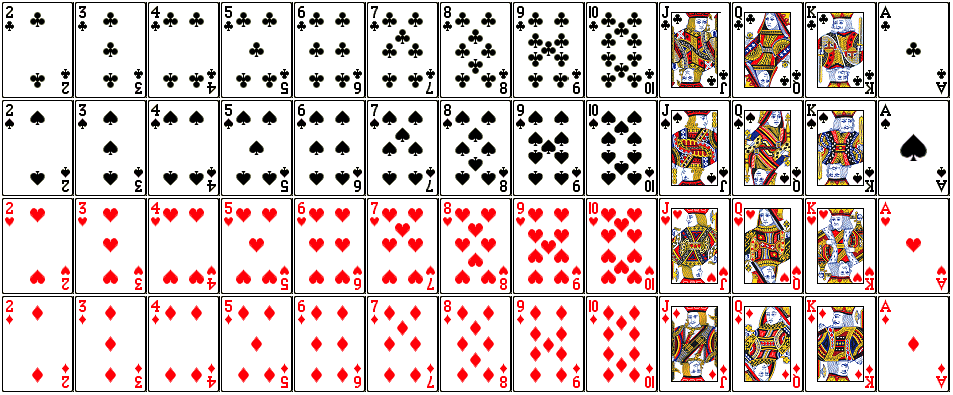
\includegraphics[scale=0.45]{kort}
\end{figure}

\prbxl{0.5}{Imagine drawing a card from a shuffled deck. We want to find the probability of 'drawing a club card \textsl{or} an honour card'. We start by counting the favorable outcomes for club cards, and find that there are 13 of them.}
\qquad
\prbxr{0.4}{A card like the club king is a club card, but it's also an honour card, so it's both; \textsl{both} a club card \textsl{and} an honour card.}

\begin{figure}[H]
	\centering
	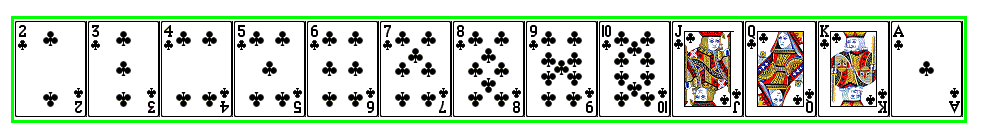
\includegraphics[scale=0.45]{kort1}
\end{figure}

Next, we count the favorable outcomes for honour cards, and find that there are 16 of them.

\begin{figure}[H]
	\centering
	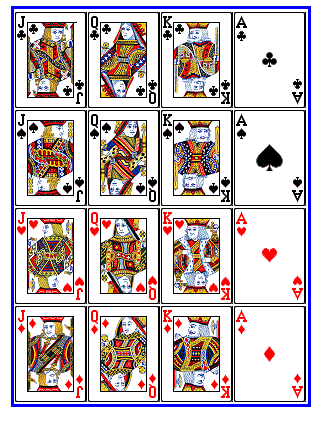
\includegraphics[scale=0.45]{kort2}
\end{figure}

In total, we've counted ${13+16=29}$ favorable outcomes, but now we encounter a problem. When we found all the club cards, we counted cards like the club jack, queen, king, and ace. These same four cards were also counted when we found all the honour cards, which means we've counted the same cards twice!

\begin{figure}[H]
	\centering
	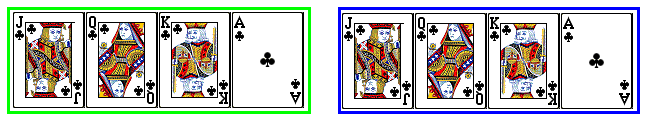
\includegraphics[scale=0.45]{kort4}
\end{figure}

For example, there aren't two club aces in a deck, so to calculate the number of cards that meet the requirement of being either a club or an honour card, we must subtract the number of cards we've counted twice:

$$ 13+16-4=25 $$

\begin{figure}[H]
	\centering
	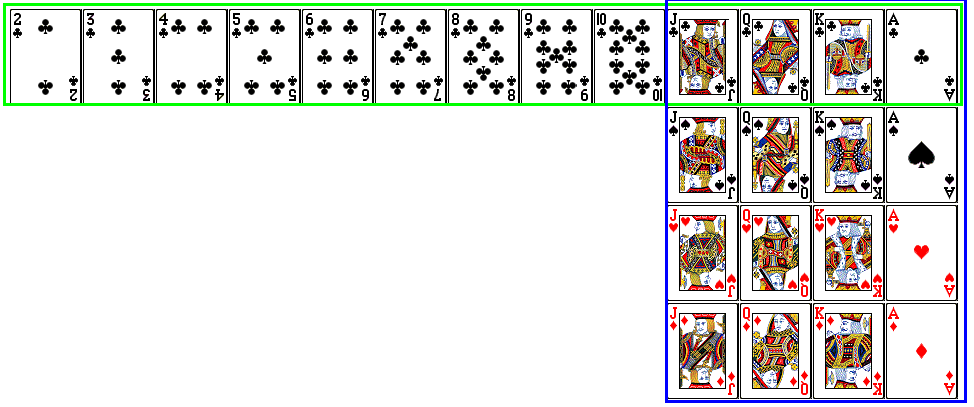
\includegraphics[scale=0.45]{kort3}
\end{figure}

Let \textit{K} be the event 'drawing a club card' and \textit{H} be the event 'drawing an honour card'. Since there are 25 cards that are either club cards \textsl{or} honour cards out of a total of 52 cards, we have

$$P(K\cup\,H)=\frac{25}{52}$$

Since we have 13 club cards and 16 honour cards, we further have

$$P(K)=\frac{13}{52} \text{ and } P(H)=\frac{16}{52}$$

\prbxl{0.6}{
	We've seen that four cards are \textsl{both} clubs \textsl{and} honour cards; this is represented as}\qquad
\prbxr{0.3}{The symbol \sym{$ \cap $} is called \textit{intersection}.} \vs

\[ K\,\cap\,H=4 \]

We then say that \textit{K} and \textit{H} have 4 common outcomes.

Furthermore, we have

\[ P(K\,\cap\,H)=\frac{4}{52} \]

Now that we've found $ P(K), P(H)$, and $P(K\cup H)$, we can find $P(K\,\cap\,H)$ again as follows:

\begin{align*}
	P(K\,\cup\,H)&=P(K)+P(H)-P(K\,\cap\,H) \br
	&= \frac{13}{52}+\frac{16}{52}-\frac{4}{52} \br
	&= \frac{25}{52}
\end{align*}

\reg[Events with common outcomes \label{mfutf}]{For two events $ A $ and $ B $,
	\[ P(A\,\cup\,B)=P(A)+P(B)-P(A\,\cap\,B) \]\vs\vs}

\info{Note}{
	If you apply \rref{mfutf} to two events without common outcomes, you end up with \rref{ufutf}. 
}

\newpage

\eks{ \label{eksfothand}
	In a class of 20 people, 7 play football, and 10 play handball. Out of these, 4 play both football and handball. If one person is randomly chosen from the class, what is the probability that this person plays football \textsl{or} handball?
	
	\sv
	Let $ F $ be the event 'plays football' and $ H $ be the event 'plays handball'.
	
	\begin{itemize} 
		\item The probability that a person plays football is
		\[ P(F)=\frac{7}{20} \]
		\item The probability that a person plays handball is
		\[ P(H)=\frac{10}{20} \]
		\item The probability that a person plays \textsl{both} football and handball is
		\[ P(F\cap H)=\frac{4}{20} \]	
	\end{itemize}
	
	Therefore, the probability that a person plays football \textsl{or} handball is 
	\begin{align*}
		P(F\cup H)&= P(F)+P(H)-P(F\cap H)\\
		&=\frac{7}{20}+\frac{10}{20}-\frac{4}{20}\\
		&=\frac{13}{20}
	\end{align*}
}
\section{Venn Diagrams}

The purpose of a Venn diagram is to create a visual representation that illustrates the count of distinct outcomes and shared outcomes. Let's use the example on page [page number] to construct such a diagram. For a class where some students play football, some play handball, and some play both, we can create a Venn diagram as shown below:

\begin{figure}[H]
	\centering
	\includegraphics[]{\figp{venn}}
\end{figure}

The green ellipse represents those who play football ($F$), and the blue ellipse represents those who play handball ($H$). Since some students play both sports ($F\cap H$), we've depicted the ellipses with a slight overlap. We know that 7 students play football, 10 play handball, and 4 of them do both, which is illustrated as follows:

\begin{figure}[H]
	\centering
	\includegraphics[]{\figp{vennb}}
\end{figure}

The diagram now shows that 3 students play football only, 6 play handball only, and 4 play both football and handball. So, a total of 7 students play football, and 10 play handball.

\eks[1]{

In a class of 31 students, 15 students take the bus to school, and 9 students take a boat. Out of these, 3 students take both the bus and the boat.

\textbf{a)} Create a Venn diagram that illustrates the given information.

\textbf{b)} If one person is randomly selected from the class, what is the probability that this person takes either the bus or the boat to school?

\textbf{Solution:}

\textbf{a)} Since 3 students take both the bus and the boat, there are 15 - 3 = 12 students who take only the bus, and 9 - 3 = 6 students who take only the boat. We can represent this using a Venn diagram:

\fig{venne}

\textbf{b)} To find the probability of selecting a student who takes either the bus or the boat, we need to calculate the total number of students who take either mode of transportation. From the diagram, we see that there are 8 students who take only the bus, 3 who take only the boat, and 3 who take both. So, there are 8 + 3 + 3 = 14 students who take either the bus or the boat. Since there are 31 students in total, the probability is:
\[
P(\text{Bus or Boat}) = \frac{14}{31}
\]
}
\eks[2]{
In a class of 29 students, we have the following information:
\begin{itemize}
	\item 16 students play football.
	\item 12 students play handball.
	\item 7 students play volleyball.
	\item 5 students play both football and handball but not volleyball.
	\item 3 students play both football and volleyball but not handball.
	\item 2 students play both handball and volleyball but not football.
	\item 1 student plays all three sports.
\end{itemize}

\textbf{a)} Create a Venn diagram that describes the distribution of the three sports in the class.

\textbf{b)} One student is randomly selected from the class. What is the probability that this student plays either football, handball, or volleyball?

\textbf{c)} The selected student turns out to play football. What is the chance that this student also plays handball?

\textbf{Solution:}

\textbf{a)} Let $F$ represent 'plays football,' $H$ represent 'plays handball,' and $V$ represent 'plays volleyball.' When creating a Venn diagram, it's a good idea to fill in the shared outcomes first. Based on the fourth to seventh points, we can draw the following:

\begin{figure}[H]
	\centering
	\includegraphics[]{\figp{venn3ea}}
\end{figure}

Next, we see that there are $16-5-1-3=7$ students who play football only, $12-5-1-2=4$ who play handball only, and $9-3-1-2=3$ who play volleyball only:

\begin{figure}[H]
	\centering
	\includegraphics[]{\figp{venn3e}}
\end{figure}

\textbf{b)} From the diagram, we can see that there are $8+5+1+3+4+2+3=26$ unique students who play one or more of the sports. The probability of selecting one of these 26 students from a class of 29 is $\frac{26}{29}$.

\textbf{c)} Reading from the diagram, out of the total 16 students who play football, there are $5+1=6$ who also play handball. Therefore, the probability that the selected student, who plays football, also plays handball is $\frac{6}{16}=\frac{3}{8}$.
}

\subsection{Cross Table}

When it comes to two events, we can also set up a \textit{cross table} to get an overview. Let's say that in a school with 300 students, milk and apples are distributed to the students who want them during lunch. Furthermore, 220 of the students receive milk, while 250 receive apples. Among them, 180 receive both milk and apples. If we let $ M $ mean \textit{receives milk} and $ E $ mean \textit{receives apples}, our cross table will initially look like this:

\begin{center}
	\renewcommand{\arraystretch}{1.5}
	\begin{tabular}{|c|c|c|c}
		& M &$ \bar{M} $ & Total \\
		\hline$ E $ & & \\
		\hline$ \bar{E} $ & &\\
		\hline Total & &
	\end{tabular}
\end{center}

Then we fill in the table based on the information we have:
\begin{itemize}
	\item Receives \textsl{both} milk and apples: \y{M\cap E = 180}
	\item Receives milk but not apples: \y{M\cap \bar{E} = 220-180=40}
	\item Receives apples but not milk: \y{E\cap M=250-180=70}
	\item Receives neither milk nor apples: \y{\bar M \cap\bar{E}=300-180-40-70=10}
\end{itemize}

\begin{center}
	\renewcommand{\arraystretch}{1.5}
	\begin{tabular}{|c|c|c|c}
		& M &$ \bar{M} $ & Total \\
		\hline$ E $ & 180& 70&250 \\
		\hline$ \bar{E} $ & 40 &10&50\\
		\hline Total & 220& 80& 300
	\end{tabular}
\end{center}

\section{Repeated Draws \label{komb}}
\subsection{Permutations}
\begin{figure}[H]
	\centering
	\includegraphics[scale=0.8]{\figp{bolle}}
	\vs
\end{figure}
Let's say we have a bowl with four balls numbered from 1 to 4. In an experiment, we draw one ball at a time until we have drawn three balls. For example, if we first draw ball 2, then ball 4, and then ball 3, we get the \textit{permutation} $2\; 4\; 3$. \vsk

How many different permutations can we get? Let's create a figure to help us find the answer. In the first draw, there are 4 balls to choose from, so we can say that we have 4 paths to take. We can either draw ball 1, ball 2, ball 3, or ball 4:
\begin{figure}[H]
	\centering
	\includegraphics[scale=0.8]{\figp{perm1a}}
\end{figure}
We remove the ball we draw from the bowl and draw again for the second time. For each of the 4 paths we could take in the first draw, we now have 3 new paths to take. So, we have a total of $3 \cdot 4 = 12$ paths we can take.

\begin{figure}[H]
	\centering
	\includegraphics[scale=0.8]{\figp{perm1b}}
\end{figure}

We also remove the second ball we draw from the bowl, and for each of the 12 paths from the second draw, we now have 2 new possible paths to take. Therefore, the total number of paths (permutations) is $12 \cdot 2 = 24$.

\begin{figure}[H]
	\centering
	\includegraphics[scale=0.8]{\figp{perm1c}}
\end{figure}

We could also express this calculation as:
\[ 4 \cdot 3 \cdot 2 = 24 \]
\textit{Rule for the product of permutations}: When we perform multiple draws in succession, we find all possible permutations by multiplying the number of possible outcomes in each draw.
\newline
\textbf{Example 1:}
Out of the 29 letters in the alphabet, we want to create a 3-letter word. We accept words that have no meaning, but each letter can only be used once in the word.
\newline
\textbf{How many words can we create?}
\newline
\textbf{Solution:}
First, we have 29 letters to draw from, then 28 letters, and finally 27 letters. Therefore, the number of permutations is given as
\[ \underbrace{29}_{\substack{\text{possible outcomes}\\\text{1st draw}}}\cdot\underbrace{28}_{\substack{\text{possible outcomes}\\\text{2nd draw}}}\cdot\underbrace{27}_{\substack{\text{possible outcomes}\\\text{3rd draw}}}=21\,924 \]
So, we can create 21\,924 different words.
\newline
\textbf{Example 2:}
We flip a coin four times in a row. How many permutations do we have?
\newline
\textbf{Solution:}
Each time we flip a coin, we have two possible outcomes. Therefore, the number of permutations is given as
\[ 2 \cdot 2 \cdot 2 \cdot 2 = 16 \]

\info{Combinations}{
	In everyday language, the word "combinations" is often used instead of "permutations," but in probability theory, combinations and permutations have different meanings. The key difference is that permutations take order into account, while combinations do not.
	
	For example, if we want to form a two-letter word using the letters $ A $, $ B $, and $ C $, and we allow the reuse of letters, then we have 9 possible permutations:
	\[ AA, AB, AC, BB, BA, BC, CC, CA, CB \]
	
	Combinations, on the other hand, refer to a unique combination when order is not considered. For example, both $ AB $ and $ BA $ are the same combination. In this case, we have 6 combinations:
	\[ AA, AB, AC, BB, BC, CC \]
}
\newpage
I can help you translate the provided Norwegian text to English while preserving LaTeX commands and not translating words starting with a backslash. Here's the translation:

```latex
\section{Probability in Repeated Draws}
\prbxl{0.5}{Imagine we have a bowl with seven balls. Three of them are green, two are blue, and two are red. Let's say we first draw one ball from the bowl, and then another. What is the probability of drawing two green balls?}\qquad
\fgbxr{0.4}{
	\fig{bolle2}
}

If we let $ G $ represent 'drawing a green ball,' we can write this probability as $ P(GG) $. To find an answer, we start by determining the number of \textsl{favorable} permutations we have. Since there are 3 favorable outcomes in the first draw and 2 in the second draw, we have $3\cdot2=6$ favorable permutations. We choose from 7 balls in the first draw and 6 balls in the second draw. Therefore, the number of \textsl{possible} permutations is $7\cdot6=42$. So, the probability of getting two green balls is
\begin{equation}
	P(GG)=\frac{3\cdot2}{7\cdot6}=\frac{6}{42}=\frac{1}{7} \label{draw}
\end{equation}
\rule{\linewidth}{1pt}
Let's also find the probability of getting a green ball in each draw separately. In the first draw, we have 3 green balls out of a total of 7 balls, so
\[ P(G)=\frac{3}{7} \]
\prbxl{0.5}{In the second draw, it is assumed that a green ball has been picked in the first draw and is therefore out of the bowl. We now have 2 out of 6 balls that are green:
	\[ P(G|G)=\frac{2}{6} \]
}
\qquad
\prbxr{0.4}{The symbol \sym{$ | $} means '\textit{\textsl{given that... has happened}}.' $ P(G|G) $ is a shorthand for 'the probability of drawing a green ball, \textsl{given that} a green ball has been drawn.'}

If we multiply the probability from the first draw by the probability from the second draw, the calculation is the same as in equation \eqref{draw}:
\[ P(GG)=\frac{3}{7}\cdot\frac{2}{6}=\frac{6}{42}=\frac{1}{7} \]

\reg[Probability in Repeated Draws]{The probability of event $ A $ happening, \textsl{given that} event $ B $ has occurred, is written as $ P(A|B) $. \vspace{5pt}
	
	The probability of events happening in sequence, such as $ A $ first, then $ B $, then $ C $, and so on ($ ... $), is given by
	\[ P(ABC...) = P(A) \cdot P(B|A) \cdot P(C|AB) \cdot... \]
}

\eks{
	In a bowl, there are 10 balls: three green, two blue, and five red. You draw two balls from the bowl. Let $ G, B, $ and $ R $ denote 'drawing a blue ball,' 'drawing a green ball,' and 'drawing a red ball,' respectively.\vspace{5pt}
	
	\textbf{a)} Draw a choice tree that outlines the permutations of $ B, G, $ and $ R $ that you can obtain.\vspace{5pt}
	\textbf{b)} What is the probability that you draw two red balls? \vspace{5pt}
	\textbf{c)} What is the probability that you draw one blue and one green ball? \vspace{5pt}
	\textbf{d)} What is the probability that you draw \textsl{at least} one blue \textsl{or} one green ball?
	
	\textbf{Solution:}\vspace{5pt}
	
	\textbf{a)}
	\begin{figure}[H]
		\centering
		\includegraphics{\figp{treee}}
	\end{figure}
	
	\textbf{b)} From our choice tree, we see that
	\alg{
		P(RR)&=\frac{2}{10}\cdot\frac{1}{9}\br
		&= \frac{2}{90} \br
		&= \frac{1}{45}
	}
	
	\textbf{c)} Both permutations $ GB $ and $ BG $ result in one blue and one green ball. The probability for each of them is
	\alg{
		P(GB)&= \frac{3}{10}\cdot\frac{5}{9} \br
		&= \frac{15}{90} \br
		&= \frac{1}{6}
	}
	\alg{
		P(BG) &= \frac{5}{10}\cdot\frac{3}{9} \br
		&= \frac{1}{6}
	}
	The probability for $ GB $ \textsl{or} $ BG $ is the sum of $ P(GB) $ and $ P(BG) $:
	\alg{
		P(GB\cup BG) &= P(GB)+P(BG) \\
		&= \frac{1}{6}+\frac{1}{6} \br
		&= \frac{2}{6} \br
		&= \frac{1}{3}
	}
	
	\textbf{d)} To answer this question, we can, of course, add the probability of the permutations $ GG, GB, GR, BG, BB, BR, RG, $ and $ RB $, but we save a lot of work by noting this: Getting \textsl{at least} one blue or one green ball is the opposite of getting \textsl{only} red balls. We found the probability of this, getting two red balls, in part b). Using \rref{complement}, we have that
	\alg{
		P(\bar{R}) &= 1-P(R) \br
		&= 1- \frac{1}{45} \br
		&= \frac{45}{45}-\frac{1}{45} \br
		&= \frac{44}{45}
	}
	So, the probability of getting \textsl{at least} one blue or one green ball is $ \frac{44}{45} $.
}

\end{document}


